\hypertarget{aircraft-handling}{%
\chapter{Aircraft handling}\label{aircraft-handling}}

\hypertarget{how-to-use-the-autopilot}{%
\section{How to use the autopilot}\label{how-to-use-the-autopilot}}

You can find the autopilot on top of your dashboard in a plane. Upon
startup it looks like this:

The autopilot has different modes you can engage or disengage by
pressing the buttons. When you change a value, the change is immediately
applied to the current mode.

\hypertarget{heading-modes}{%
\subsection{Heading modes}\label{heading-modes}}

HDG (Heading): set the airplane heading to the heading selected (in
degree)

WLV (Wing Leveler): set the wings horizontal. The airplane should
roughly keep its current heading.

NAV (Radio Navigation): engage when approaching a runway equipped with
an ILS equipment (the red and white antennas). The airplane will first
try to intercept the runway axis, then stay along it until you pass the
runway edge.

\hypertarget{heading-listings}{%
\subsubsection{Heading Listings}\label{heading-listings}}

This is a list of headings to use for ILS on included maps.

North St.~Helens main runway - 240 degrees

Aspen main runway - 190 degrees

\hypertarget{altitude-modes}{%
\subsubsection{Altitude modes}\label{altitude-modes}}


\includegraphics{images/autopilot-alt.jpg}

HOLD (Hold altitude): set the altitude to the altitude selected (in
feet). The the maximum vertical speed allowed to reach the altitude is
selected by the vert.speed setting (in feet per minute, the sign of the
selected vert speed is ignored). So this mode works better with a
vert.speed different than 0!

V/S (Vertical Speed): set the vertical speed (in feet per minute),
without a target altitude. Positive value to climb, negative to descent.

NAV+V/S (Vertical Radio Navigation): when both NAV and V/S are selected,
the altitude is controlled by the ILS system. So when approaching a
runway with NAV, engage V/S to make the plane descend to the runway.

\hypertarget{speed-mode}{%
\subsubsection{Speed mode}\label{speed-mode}}

ATHR (Auto-Throttles) set the speed of the airplane as selected in IAS
(Indicated Air Speed, in knots).

\hypertarget{other-buttons}{%
\subsubsection{other buttons}\label{other-buttons}}

GPWS (Ground Proximity Warning System): when engaged, a recorded voice
calls altitude and warns in case of dangerous maneuvers close to the
ground.

BRKS (Parking brakes)

\hypertarget{horizontal-navigation-indicator-hsi}{%
\subsection{Horizontal Navigation Indicator
(HSI)}\label{horizontal-navigation-indicator-hsi}}

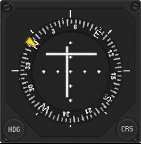
\includegraphics{images/autopilot-hsi.jpg}

There is a simplified HSI (Horizontal Navigation Indicator) instrument
between the AOA (Angle of Approach) indicator and the engine gauges. It
includes:

a compass

a heading bug (that runs along the heading selector)

two position indicators:

a vertical bar for horizontal deviation

a horizontal bar for vertical deviation.

They tell you how far you are from the optimal trajectory when you do an
ILS approach. The optimal position is when both bars are at the center
of the display.

\hypertarget{how-to-do-a-successful-instruments-approach-with-the-ils}{%
\subsection{How to do a successful instruments approach with the
ILS}\label{how-to-do-a-successful-instruments-approach-with-the-ils}}

ensure the approach you want to do is equipped with an ILS:

check if there are red and white antennas at the end of the runway, at
the side where you will touch down. Be sure the approach is clear of
obstacles.

fly to a comfortable distance from the runway, preferably off the
terrain.

ensure you are at the right altitude for an approach from that distance.
If the horizontal bar is low, descend, if it is high, climb.

fly in a way so you will soon intercept the runway axis, or are roughly
on the runway axis

Engage NAV, then V/S. Drop the joystick. The plane should fly by itself
now, intercepting the runway axis and descending to the runway.

You can see how it performs on the HSI display. The bars should cross at
the center when the approach is stabilized.

Control your speed! You should fly as slow as possible (around 100 knots
for the Antonov 12). Use auto-throttle if possible. Watch the AOA, if it
gets too high, you will stall! Add more flaps in that case.

If you go too fast, the plane will not descend and the horizontal bar
will go down.

On short final, the GPWS calls ``Minimums'': you reached the minimum
decision altitude. If you see the runway and everything is fine, proceed
to the landing (real pilots disconnect the autopilot at this stage and
land by the hand).

The autopilot should disconnect at the runway edge, but in some case it
can continue to function, so be cautious at the flare.

Engage reverses and brake (press and maintain key B). You landed!
